%% LyX 2.3.4.2 created this file.  For more info, see http://www.lyx.org/.
%% Do not edit unless you really know what you are doing.
\documentclass[UTF8]{ctexart}
\usepackage[T1]{fontenc}
\usepackage{geometry}
\geometry{verbose,tmargin=3cm,bmargin=3cm,lmargin=2cm,rmargin=2cm,headheight=1cm,headsep=1cm}
\usepackage{fancyhdr}
\pagestyle{fancy}
\usepackage{float}
\usepackage{graphicx}

\makeatletter
%%%%%%%%%%%%%%%%%%%%%%%%%%%%%% User specified LaTeX commands.
% 如果没有这一句命令,XeTeX会出错,原因参见
% http://bbs.ctex.org/viewthread.php?tid=60547
\DeclareRobustCommand\nobreakspace{\leavevmode\nobreak\ }

\makeatother

\begin{document}
\title{转移矩阵}
\date{任杰}
\maketitle

\section{一维经典伊辛模型}

转移矩阵的概念最早是在处理经典伊辛模型中引入的,因此我们从最简单的一维经典伊辛模型为例引入转移矩阵的概念。考虑一个 N 格点周期边界系统:

\begin{equation}
H=-J\sum_{i}s_{i}s_{i+1},
\end{equation}
我们处理的是一个经典统计问题。考虑配分函数:

\begin{equation}
Z=\sum_{\left\{ s_{i}\right\} }\prod_{i}\exp\left(Ks_{i}s_{i+1}\right),
\end{equation}
其中 $K=J/kT$. 注意到配分函数可以写为一个乘积形式:

\begin{equation}
Z=Tr\left(T^{N}\right),
\end{equation}
\begin{equation}
T_{ss'}=e^{Kss'}=\left(\begin{array}{cc}
e^{K} & e^{-K}\\
e^{-K} & e^{K}
\end{array}\right).
\end{equation}
由此引入的矩阵就是我们将要介绍的转移矩阵。我们将要说明,转移的本征谱可以给出系统的统计信息。

\subsection{转移矩阵谱与临界点}

我们首先给出 T 的谱分解:

\begin{equation}
T=\lambda_{0}\left|0\right\rangle \left\langle 0\right|+\lambda_{1}\left|1\right\rangle \left\langle 1\right|,
\end{equation}
其中

\begin{equation}
\lambda_{0},\lambda_{1}=2\cosh K,2\sinh K,
\end{equation}

\begin{equation}
\left|0\right\rangle ,\left|1\right\rangle =\frac{1}{\sqrt{2}}\left(\begin{array}{c}
1\\
\pm1
\end{array}\right)
\end{equation}
回到原来的问题。得到转移矩阵 T 的谱之后(往往我们只会用到本征值),我们可以计算配分函数:

\begin{eqnarray}
Z & = & \left\langle 0\right|T^{N}\left|0\right\rangle +\left\langle 1\right|T^{N}\left|1\right\rangle \nonumber \\
 & = & \lambda_{0}^{N}+\lambda_{1}^{N}\nonumber \\
 & = & \lambda_{0}^{N}\left[1+\left(\frac{\lambda_{1}}{\lambda_{0}}\right)^{N}\right]\nonumber \\
 & = & \left(2\cosh K\right)^{N}\left[1+\tanh^{N}K\right].
\end{eqnarray}
从配分函数的形式中,我们看到当我们取热力学极限:$N\rightarrow\infty$ 时, $Z\rightarrow\left(2\cosh K\right)^{N}$。热力学极限下的平均自由能

\begin{equation}
f:=-\lim_{N\rightarrow\infty}\frac{1}{N}\ln Z=-2\ln\lambda_{0}.
\end{equation}
完全来自于转移矩阵的基态。当我们改变温度,若转移矩阵的本征值发生交叉,体系自由能在交叉处就会有非解析性,该临界点就发生了热力学相变。转移矩阵谱的简并意味着相变临界点,对于我们现在讨论的模型,有限温度时总是有
$\lambda_{0}>\lambda_{1}$,即一维经典伊辛模型只有一个相。

\subsection{转移矩阵谱与关联长度}

在继续我们的讨论之前。考虑格点算符 $O_{i}$ 关联函数(设 $i<j$):

\begin{eqnarray}
\left\langle O_{i}O_{j}\right\rangle  & = & \frac{Tr\left[ZO_{i}O_{j}\right]}{Tr\left[Z\right]}\nonumber \\
 & = & \frac{Tr\left[T^{N}O_{i}O_{j}\right]}{Tr\left[T^{N}\right]}\nonumber \\
 & = & \frac{Tr\left[T^{i}O_{i}T^{j-i}O_{j}T^{N-j}\right]}{Tr\left[T^{N}\right]}.
\end{eqnarray}
此形式类似编时关联函数。实际上,以转移矩阵作为桥梁,我们可以将一个 d 维经典统计问题和一个 d - 1 维量子统计问题相互转化,我们会在以后讨论这个问题。这里,我们写出分母低阶表达式:

\begin{equation}
Tr\left[T^{i}O_{i}T^{j-i}O_{j}T^{N-j}\right]\approx\lambda_{0}^{N}\left[\left\langle 0\right|O_{i}\left|0\right\rangle \left\langle 0\right|O_{j}\left|0\right\rangle +\left(\frac{\lambda_{1}}{\lambda_{0}}\right)^{j-i}\left\langle 0\right|O_{i}\left|1\right\rangle \left\langle 1\right|O_{j}\left|0\right\rangle \right].
\end{equation}
\begin{eqnarray}
\left\langle O_{i}O_{j}\right\rangle _{c} & = & \left\langle O_{i}O_{j}\right\rangle -\left\langle O_{i}\right\rangle \left\langle O_{j}\right\rangle \nonumber \\
 & = & \left(\frac{\lambda_{1}}{\lambda_{0}}\right)^{j-i}\left\langle 0\right|O_{i}\left|1\right\rangle \left\langle 1\right|O_{j}\left|0\right\rangle .
\end{eqnarray}
关联长度由 $\lambda_{1}/\lambda_{0}$ 确定。这从另一个角度说明相变临界点物理意义,即无穷关联长度。对于一维情形,取
$O_{i}=s_{i}$:

\begin{equation}
\left\langle s_{i}s_{j}\right\rangle =\left(\tanh K\right)^{\left|i-j\right|}.
\end{equation}


\subsection{转移矩阵联系经典与量子系统}

在这一步,我们在原来体系中引入磁场:

\begin{equation}
H=-J\sum_{i}s_{i}s_{i+1}-h\sum_{i}s_{i},
\end{equation}

\begin{equation}
Z=\sum_{\left\{ s_{i}\right\} }\prod_{i}\exp\left(Ks_{i}s_{i+1}\right)\cdot\prod_{i}\exp\left(Hs_{i}\right),
\end{equation}
其中 $K=J/kT,H=h/kT$. 利用类似的方法,定义:

\begin{equation}
V_{ss'}^{(1)}=\exp\left(Kss'\right)\propto\exp\left(K^{*}\sigma^{x}\right)_{ss'},
\end{equation}

\begin{equation}
V^{(2)}=\exp\left(H\sigma^{z}\right),
\end{equation}
其中 $\tanh K^{*}=e^{-2K}.$ 注意这里 $V^{(1)},V^{(2)}$ 的定义方式有所不同,$V^{(1)}$
定义式中 s 作为脚标,$V^{(2)}$定义中 s 被看作算符本身($\sigma^{z}$),两种方式得到的矩阵往往是非对易的,这是转移矩阵“量子”的来源。转移矩阵现在可以写为:

\begin{equation}
T=\sqrt{V^{(2)}}V^{(1)}\sqrt{V^{(2)}},
\end{equation}
其中我们将 $V^{(2)}$ 拆为 2 半以使转移矩阵是厄米的,这样定义的转移矩阵同样满足:

\begin{equation}
Z=Tr\left[T^{N}\right].
\end{equation}
若 $K^{*},H\ll1$,我们可以交换矩阵位置:

\begin{equation}
T\approx V^{(1)}V^{(2)}=\exp\left[-\frac{\beta}{N}\left(-\sigma^{x}-\frac{h}{K^{*}}\sigma^{z}\right)\right],
\end{equation}
其中 $\beta=KN$,也就是说,转移矩阵对应一个 0 维量子系统

\begin{equation}
\mathcal{H}=-\sigma^{x}-\frac{h}{K^{*}}\sigma^{z}
\end{equation}
的虚时演化。现在回头看上一节中伊辛模型关联函数:

\begin{eqnarray}
\left\langle O_{i}O_{j}\right\rangle  & = & \frac{Tr\left[T^{i}O_{i}T^{j-i}O_{j}T^{N-j}\right]}{Tr\left[T^{N}\right]}\nonumber \\
 & = & \frac{Tr\left[e^{-\beta\mathcal{H}}O\left(\tau_{i}\right)O\left(\tau_{j}\right)\right]}{Tr\left[e^{-\beta\mathcal{H}}\right]},
\end{eqnarray}
其中我们定义:

\begin{equation}
O\left(\tau_{i}\right)=T^{-i}OT^{i}=e^{\frac{\beta}{N}i}Oe^{-\frac{\beta}{N}i},
\end{equation}
这正是定义在有限温度量子体系中的松原函数。

再次总结该模型中得到的结果。我们从一维经典统计系统的配分函数出发,将配分函数分割成 N 个转移矩阵的乘积,这 N 个乘积正对应了统计系统的一个维度。这样,转移矩阵对应少一个维度的体系虚时演化,我们可以由此得到一个
1 - 1 维(量子)系统。而此量子系统的松原函数对应经典系统关联函数。同时,热力学相变临界点对应转移矩阵谱基态简并,而这正对应 1
- 1 维量子体系能隙关闭处,因此,d - 1 维量子体系量子临界点对应 d 维经典体系热力学临界点。0 维量子体系不存在相变,这也佐证了
1 维经典伊辛模型只有一个相的结论。

\section{二维经典伊辛模型}

一维模型作为例子足够说明转移矩阵的性质。但一维经典体系没有相变,更加非平庸的结论存在于二维体系中。考虑二维经典伊辛模型($N\times M$):

\begin{equation}
H=-J_{\tau}\sum_{i,j}s_{i,j}s_{i,j+1}-J_{x}\sum_{i,j}s_{i,j}s_{i+1,j}.
\end{equation}
配分函数为:

\begin{equation}
Z=\sum_{\left\{ s_{i,j}\right\} }\prod_{i,j}exp\left(K_{\tau}s_{i,j}s_{i,j+1}\right)\cdot\prod_{i,j}\exp\left(K_{x}s_{i,j}s_{i+1,j}\right).
\end{equation}
配分函数和一维情形基本一致,只是扩展了一个维度。这时,转移矩阵代表一行 N 个矩阵指标:

\begin{equation}
V^{(1)}\left(s_{1},\cdots,s_{N};s'_{1},\cdots,s'_{N}\right)=\prod_{i}exp\left(K_{\tau}s_{i}s'_{i}\right)\propto\exp\left(K_{\tau}^{*}\sum_{i}\sigma_{i}^{x}\right),
\end{equation}

\begin{equation}
V^{(2)}=\exp\left(K_{x}\sum_{i}\sigma_{i}^{z}\sigma_{i}^{z}\right),
\end{equation}
同样 $\tanh K_{\tau}^{*}=e^{-2K_{\tau}}$. 重复以上的讨论,转移矩阵最终对应到一个一维量子哈密顿量:

\begin{equation}
\mathcal{H}=-\sum_{i}\sigma_{i}^{x}-\frac{K_{x}}{K_{\tau}^{*}}\sum_{i}\sigma_{i}^{z}\sigma_{j}^{z},
\end{equation}
这正是一维量子横场伊辛模型。该模型量子临界点在

\begin{equation}
\frac{K_{x}}{K_{\tau}^{*}}=1
\end{equation}
处。若 $J_{x}=J_{\tau}$:

\begin{equation}
K=K^{*},
\end{equation}

\begin{equation}
e^{-2K}=\tanh K,
\end{equation}

\begin{equation}
K=\frac{1}{2}\ln\left(1+\sqrt{2}\right)=\frac{J}{kT}.
\end{equation}
我们由此得到二维伊辛模型临界温度:

\begin{equation}
\frac{kT}{J}=\frac{2}{\ln\left(1+\sqrt{2}\right)}\approx2.269.
\end{equation}


\section{零温转移矩阵与量子相变}

对热力学系统,配分函数实际是密度矩阵

\begin{equation}
\rho=\sum_{n}e^{-\beta E_{n}}\left|n\right\rangle \left\langle n\right|,
\end{equation}

\begin{equation}
Z=Tr\left[\rho\right]
\end{equation}
对于处在零温的量子系统,密度矩阵就是基态。此时配分函数就是态内积,由此可以将转移矩阵的概念拓展到零温量子系统。这时直观的图像可以用矩阵乘积态表述:

\begin{figure}[H]
\begin{centering}
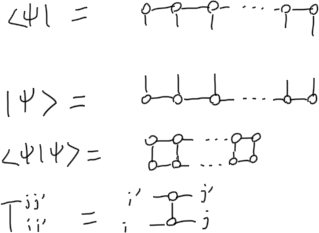
\includegraphics[width=8cm]{include/mpstrm}
\par\end{centering}
\caption{MPS 转移矩阵}

\end{figure}

\begin{flushleft}
关联函数也有类似形式:
\par\end{flushleft}

\begin{figure}[H]
\begin{centering}
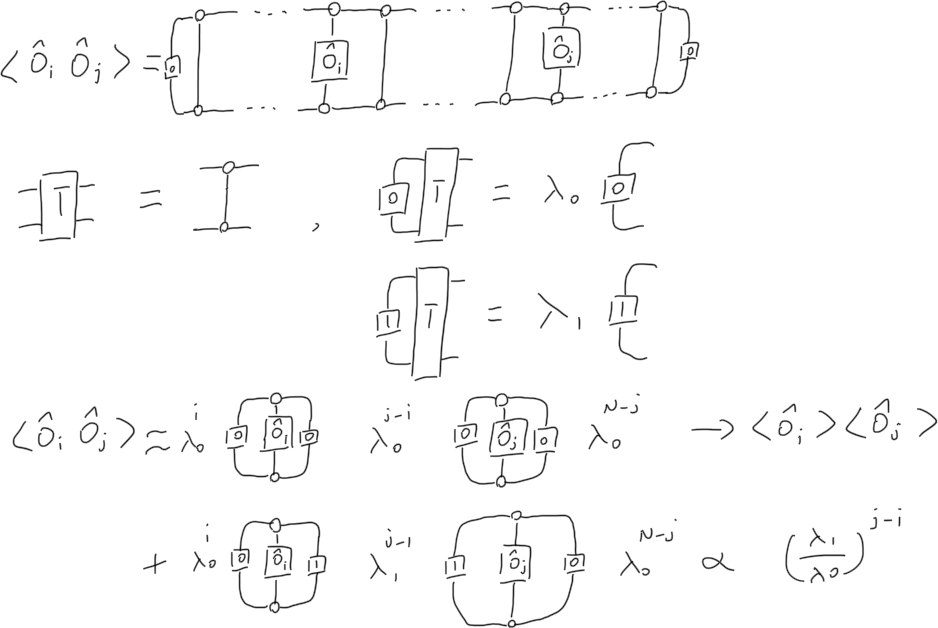
\includegraphics[width=16cm]{include/mpscor}
\par\end{centering}
\caption{MPS 关联函数}
\end{figure}

同样,量子相变临界点对应转移矩阵基态简并。
\end{document}
